%\setchapterimage{fig_02}
\chapter*{TD \arabic{cptTD} :
Stabilisateur vertical pour appareil photo \ifnormal $\star$ \else \fi \ifdifficile $\star\star$ \else \fi \iftdifficile $\star\star\star$ \else \fi
 -- \ifprof Corrigé \else Sujet \fi}
\addcontentsline{toc}{section}{TD \arabic{cptTD} : 
Stabilisateur vertical pour appareil photo \ifnormal $\star$ \else \fi \ifdifficile $\star\star$ \else \fi \iftdifficile $\star\star\star$ \else \fi
 -- \ifprof Corrigé \else Sujet \fi}

\iflivret \stepcounter{cptTD} \else
\ifprof  \stepcounter{cptTD} \else \fi
\fi

\setcounter{question}{0}
\marginnote{Concours Centrale Supelec 2021 -- PSI.}
\marginnote{
\UPSTIcompetence[2]{B2-14}
\UPSTIcompetence[2]{C1-05}
\UPSTIcompetence[2]{C2-07}
}

\begin{marginfigure}
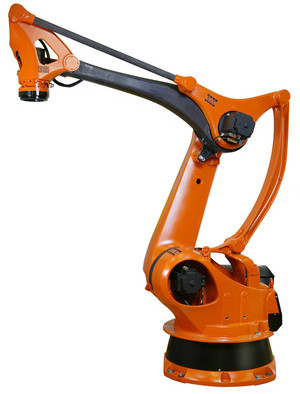
\includegraphics[width=\linewidth]{fig_01}
\end{marginfigure}

\ifprof
\else
L’utilisation du mode vidéo, en haute définition sur les appareils photo réflex et légers, pose aux photographes le problème de la stabilisation de l’image. 
 
Les nacelles gyrostabilisées, installées sur une perche portée par les
 deux mains de l’utilisateur et sur lesquelles se fixe l’appareil photographique permettent de corriger les perturbations dues aux mouvements de l’utilisateur selon trois axes de rotations. Néanmoins, elles ne permettent pas de réduire les perturbations verticales dues à la marche ou à la course de l’utilisateur.

Pour résoudre ce problème, un constructeur commercialise un stabilisateur vertical à installer entre la perche et la nacelle gyrostabilisée.

\fi

\section*{Vérification du respect de l'exigence relative à la position d'équilibre }


\ifprof
\else
Le cahier des charges précise que le stabilisateur peut être utilisé avec des appareils photo de masse comprise entre \SI{0,350}{kg} et \SI{1,550}{kg}\sidenote{Exigence 1}.
\begin{marginfigure}
\centering
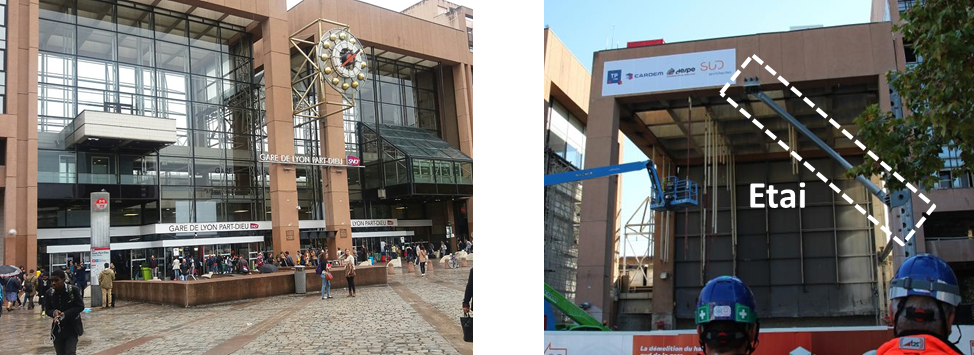
\includegraphics[width=.8\linewidth]{fig_03}
\caption{Exigence 1.1}
\end{marginfigure}
\fi

\begin{obj}
 L'objectif de cette partie est de vérifier que la conception est assez robuste vis-à-vis du facteur de masse de l'appareil photo pour satisfaire l'exigence 1.1 relative à la position d'équilibre du système.
\end{obj}

\ifprof
\else

\begin{figure}[!h]
\centering
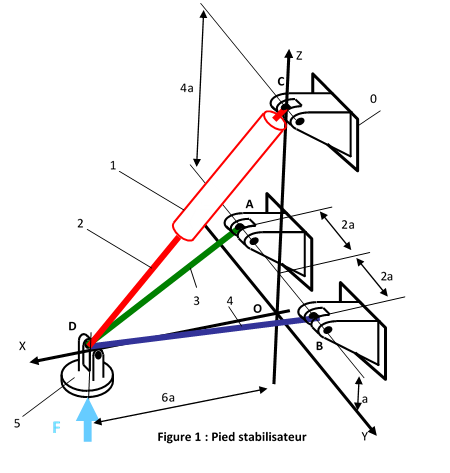
\includegraphics[width=.7\textwidth]{fig_02}
\caption{Schéma cinématique plan et paramétrage du mécanisme}
\label{Cy_11_Ch_03_PFS_2D_TD_05_fig_02}
\end{figure}


%Le mécanisme étudié dont la modélisation retenue est donnée (figure \ref{Cy_11_Ch_03_PFS_2D_TD_05_fig_02}) est principalement constitué de quatre solides $\left\{(1),(2),\left(2^{\prime}\right),(3)\right\}$ formant un parallélogramme et guidés deux à deux en rotation par des liaisons modélisées par des pivots aux points $A$, $A'$, $B$ et $B'$. La nacelle gyrostabilisée est schématisée par la barre $(3)$. Le support $(1)$, faisant l'objet d'une liaison encastrement avec la perche, est supposé être en mouvement de translation par rapport au sol $(0)$ autorisé par une glissière fictive. Ce modèle est paramétré par:

Le mécanisme étudié dont la modélisation retenue est donnée (figure \ref{Cy_11_Ch_03_PFS_2D_TD_05_fig_02}). La nacelle gyrostabilisée est schématisée par la barre $(3)$. Le support $(1)$, faisant l'objet d'une liaison encastrement avec la perche, est supposé être en mouvement de translation par rapport au sol $(0)$ autorisé par une glissière fictive. Ce modèle est paramétré par:

\marginnote{
La plage de fonctionnement du mécanisme est limitée par la géométrie des bras (2) et (2') avec $\alpha \in\left[-35^{\circ}, 45^{\circ}\right]$, $l=25 \mathrm{~mm}, L=52 \mathrm{~mm}, y_{G}=5 \mathrm{~mm}$ et $z_{G}=200 \mathrm{~mm}$.
}

\begin{itemize}
  \item le repère terrestre $\mathcal{R}_{0}\left(\mathrm{O}, \vec{x}_{0}, \vec{y}_{0}, \vec{z}_{0}\right)$ supposé galiléen avec $\vec{z}_{0}$ vertical ascendant ;

  \item le repère $\mathcal{R}_{1}\left(\mathrm{~A}, \vec{x}_{0}, \vec{y}_{0}, \vec{z}_{0}\right)$ lié au support (1) avec $\overrightarrow{\mathrm{OA}}=y_{A} \vec{y}_{0}+z_{\text {pert }} \vec{z}_{0}$;

  \item le repère $\mathcal{R}_{2}\left(\mathrm{~A}, \vec{x}_{0}, \vec{y}_{2}, \vec{z}_{2}\right)$ lié au bras (2) avec $\alpha=\left(\vec{y}_{0}, \vec{y}_{2}\right)=\left(\vec{z}_{0}, \vec{z}_{2}\right)$;

  \item le repère $\mathcal{R}_{2}^{\prime}\left(\mathrm{A}^{\prime}, \vec{x}_{0}, \vec{y}_{2}, \vec{z}_{2}\right)$ lié au bras (2') avec $\overrightarrow{\mathrm{AA}^{\prime}}=l \vec{z}_{0}$;

  \item le repère $\mathcal{R}_{3}\left(\mathrm{~B}, \vec{x}_{0}, \vec{y}_{0}, \vec{z}_{0}\right)$ lié à la nacelle gyrostabilisée (3) et à l'appareil photo (4) liés rigidement entre eux avec $\overrightarrow{\mathrm{AB}}=L \vec{y}_{2}$. Le centre d'inertie de l'ensemble $\{(3)+(4)\}$ est noté $\mathrm{G}$, avec $\overrightarrow{\mathrm{BG}}=y_{G} \vec{y}_{0}+z_{G} \vec{z}_{0} ;$

  \item le repère $\mathcal{R}_{5}\left(\mathrm{~A}^{\prime}, \vec{x}_{0}, \vec{y}_{5}, \vec{z}_{5}\right)$ est défini tel que $\overrightarrow{\mathrm{A}^{\prime} \mathrm{B}}=L_{r} \vec{y}_{5}$ avec $\beta=\left(\vec{y}_{0}, \vec{y}_{5}\right)=\left(\vec{z}_{0}, \vec{z}_{5}\right)$.

\end{itemize}




Le ressort de traction (5) de raideur $K_{r}$ et de longueur à vide $L_{r 0}$ possède une tension initiale $F_{r 0}$ lorsque $L_{r}=L_{r 0}$. Il est relié d'une part au support (1) et d'autre part au solide (3) aux points d'ancrage respectivement A' et B.

Pour cette étude la nacelle gyrostabilisée (3) et l'appareil photo (4) sont considérés comme formant un seul solide de masse $m_{34}=m_{3}+m_{4}$ avec $m_{3}=1,250 \mathrm{~kg}$. La masse et l'inertie des autres solides sont négligés.

%\begin{itemize}
%  \item la nacelle gyrostabilisée (3) et l'appareil photo (4) sont considérés comme formant un seul solide ;
%
%  \item la masse et les inerties des solides sont négligées mis à part pour l'ensemble constitué de la nacelle gyrostabilisée (3) et de l'appareil photo (4) de masse $m_{34}=m_{3}+m_{4}$ avec $m_{3}=1,250 \mathrm{~kg}$ la masse de la nacelle gyrostabilisée (3) et $m_{4}$ la masse de l'appareil photo (4).
%\end{itemize}
% La référence retenue pour décrire la position de l'appareil photo est le centre d'inertie $\mathrm{G}$ de l'ensemble constitué de la nacelle gyrostabilisée (3) et de l'appareil photo (4) dans le repère $\mathcal{R}_{0}$.
 
 
 
 \marginnote{
Dans cette partie, l'étude est conduite avec les hypothèses suivantes :
\begin{itemize}
%  \item les quatre liaisons pivots et la liaison glissière sont parfaites ;
  \item les liaisons sont parfaites ;
  \item la modélisation est plane ;
  \item il n'y pas de perturbation $\left(z_{\text {pert }}=0\right)$.
\end{itemize}}






En utilisant une fermeture géométrique, on peut montrer que $\tan\beta = \dfrac{L\sin\alpha-l}{L\cos\alpha}$ et que la longueur du ressort $L_r$ peut s'exprimer sous la forme
$L_r = \sqrt{L^2+l^2-2Ll\sin\alpha}$. 

\fi

%%Q 3. 
%\question{\label{q:03} Exprimer les coordonnées du centre d'inertie $\mathrm{G}$ dans le repère $\mathcal{R}_{0}$ en fonction de l'angle $\alpha$ et des paramètres géométriques du système.}
%\ifprof
%\begin{corrige}
%Exprimons le vecteur $\vect{OG}$ dans la base $\base{x_0}{y_0}{z_0}$.
%
%\begin{align*}
%\vect{OG} &=\vect{OA}+\vect{AB}+\vect{BG} \\
%&=y_A\vect{y_0}+z_{\text{pert}}\vect{z_0}+L\vect{y_2}+y_G\vect{y_0}+z_{G}\vect{z_0}\\
%&=y_A\vect{y_0}+z_{\text{pert}}\vect{z_0}+L\left(\cos\alpha\vect{y_0}+\sin\alpha\vect{z_0}\right)+y_G\vect{y_0}+z_{G}\vect{z_0}\\
%\end{align*}
%
%Soit au final, 
%$\vect{OG} =\left(y_A+y_G+L\cos\alpha\right)\vect{y_0}+\left(z_{\text{pert}}+z_{G}+L\sin\alpha\right)\vect{z_0}$.
%\end{corrige}
%\else
%\fi
%
%%Q 4. 
%\question{\label{q:04} En utilisant une fermeture géométrique, donner l'expression de l'angle $\beta$ en fonction de l'angle $\alpha$ et des paramètres géométriques $L$ et $l$ du système.}
%\ifprof
%\begin{corrige}
%Dans le triangle $AA'B$ on a $\vect{AA'}+\vect{A'B}+\vect{BA}=\vect{0}$. 
%En conséquence,  $l\vect{z_0}+L_r\vect{y_5}-L\vect{y_2}=\vect{0}$.
%
%On projette cette équation dans $\rep{0}$ et on a : 
% $l\vect{z_0}+L_r\left(\cos\beta\vect{y_0}+\sin\beta\vect{z_0}\right)-L\left(\cos\alpha\vect{y_0}+\sin\alpha\vect{z_0}\right)=\vect{0}$.
% 
% On a donc les équations scalaires suivantes : 
% $\left\{
% \begin{array}{l}
%L_r\cos\beta-L\cos\alpha={0}\\
% l+L_r\sin\beta-L\sin\alpha={0} \\
% \end{array}
% \right.
% $. 
% 
% On cherche à exprimer $\beta$ en fonction de $\alpha$ et donc à supprimer $L_r$; donc : 
%  $\left\{
% \begin{array}{l}
% L_r\sin\beta=L\sin\alpha-l \\
% L_r\cos\beta=L\cos\alpha\\
% \end{array}
% \right.
% $. 
% 
% En conséquence, $\boxed{\tan\beta = \dfrac{L\sin\alpha-l}{L\cos\alpha}}$.
%\end{corrige}
%\else
%\fi

%%Q 5. 
%\question{\label{q:05}Exprimer la longueur $L_{r}$ du ressort de traction (5) en fonction de l'angle $\alpha$ et des paramètres géométriques du système.}
%\ifprof
%\begin{corrige}
%En réutilisant le système d'équation précédent, on a $L_r^2 = \left(L\sin\alpha-l\right)^2+L^2\cos^2\alpha$ soit:
%
%$$\boxed{L_r = \sqrt{L^2+l^2-2Ll\sin\alpha}}.$$
%\end{corrige}
%\else
%\fi

\subsection*{Vérification de l'exigence relative à la plage de fonctionnement}
\ifprof
\else
L'action mécanique du ressort de traction (5) sur la nacelle gyrostabilisée (3) est modélisée par le torseur $\left\{\mathcal{F}_{5 \rightarrow 3}\right\}$ : 
$
\left\{\mathcal{F}_{5 \rightarrow 3}\right\}=\left\{\begin{array}{c}
F_{r} \vec{y}_{5} \\
\overrightarrow{0}
\end{array}\right\}_{\mathrm{B}} .
$
\fi

%Q 6.
\question{\label{q:06}Exprimer la composante de résultante d'action mécanique $F_{r}$ en fonction de l'angle $\alpha$, des paramètres géométriques du système et des paramètres du ressort.}
\ifprof
\begin{corrige}
En utilisant la définition de la force de rappel du ressort de traction (en tension ici) et  avec $L_{r0}$ la longueur à vide du ressort on a $F_r\vect{y_5}=-K_r\left(L_r-L_{r0}\right)\vect{y_5}$. En utilisant l'expression précédente:
 $\boxed{F_r=-K_r\left(\sqrt{L^2+l^2-2Ll\sin\alpha}-L_{r0}\right)}$.

Avec la définition de l'effort de traction donnée par l'énoncé, on peut aussi être tenté d'écrire 

$F_r\vect{y_5}=-\left[ F_{r0} + K_r\left(L_r-L_{r0}\right)\right]\vect{y_5}$. En utilisant l'expression précédente:
$\boxed{F_r=-\left[F_{r0} + K_r\left(\sqrt{L^2+l^2-2Ll\sin\alpha}-L_{r0}\right)\right]}$.
\end{corrige}
\else
\fi

%Q 7. 
\question{\label{q:07}Déterminer la direction des actions mécaniques de liaison exercées par le bras (2) sur la nacelle (3) et par le bras (2') sur la nacelle (3) \textbf{On pourra raisonner en statique)}.}
\ifprof
\begin{corrige}
Il est fait l'hypothèse que le problème est plan dans le plan $\left(0,\vect{y_0},\vect{z_0}\right)$. Les torseurs d'actions mécaniques associés aux liaisons pivot d'axe $\vect{z_0}$ sont donc des glisseurs. 

Les solides (2) et (2') sont tous soumis à deux glisseurs :
\begin{itemize}
\item d'une part, $\torseurstat{F}{1}{2}$ (pivot d'axe $\axe{A}{x_0}$) et $\torseurstat{F}{3}{2}$ (pivot d'axe $\axe{B}{x_0}$) sont des glisseurs ;
\item d'autre part, $\torseurstat{F}{1}{2'}$ (pivot d'axe $\axe{A'}{x_0}$)et $\torseurstat{F}{3}{2'}$  (pivot d'axe $\axe{B'}{x_0}$) sont des glisseurs.
\end{itemize}

D'après le PFS appliqué successivement à (2) et (2'), solides soumis à deux glisseurs, alors on a 
 $\torseurstat{F}{3}{2}+\torseurstat{F}{1}{2}=\{0\}$ et
  $\torseurstat{F}{3}{2'}+\torseurstat{F}{1}{2'}=\{0\}$. Les actions mécaniques sont de même norme, de même direction (droites $(AB)$ et $(A'B')$ soit vecteur $\vect{y_2}$).
  
De plus, $\boxed{\vect{F}_{23}=F_{23}\vect{y_2}}$ et $\boxed{\vect{F}_{2'3}=F_{2'3}\vect{y_2}}$.
\end{corrige}
\else
\fi

%Q 8. 
\question{\label{q:08}Afin de déterminer la position d'équilibre de l'ensemble $\{(3)+(4)\}$, proposer sans calcul, une démarche claire qui permette d'exprimer l'effort nécessaire du ressort de traction (5) sur la nacelle gyrostabilisée (3) \textbf{On pourra raisonner en statique)}.}
\ifprof

\begin{marginfigure}
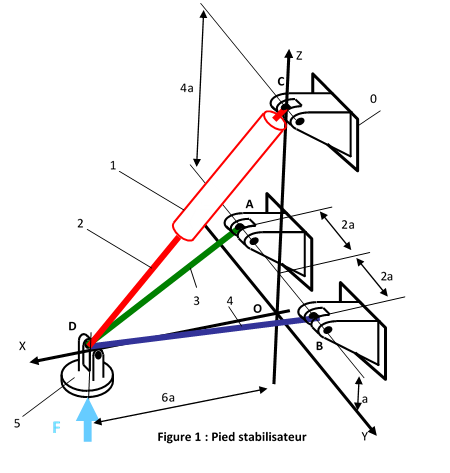
\includegraphics[width=\textwidth]{fig_02}
\caption{Rappel -- Schéma cinématique plan et paramétrage du mécanisme}
\end{marginfigure}

\begin{corrige}
\begin{center}
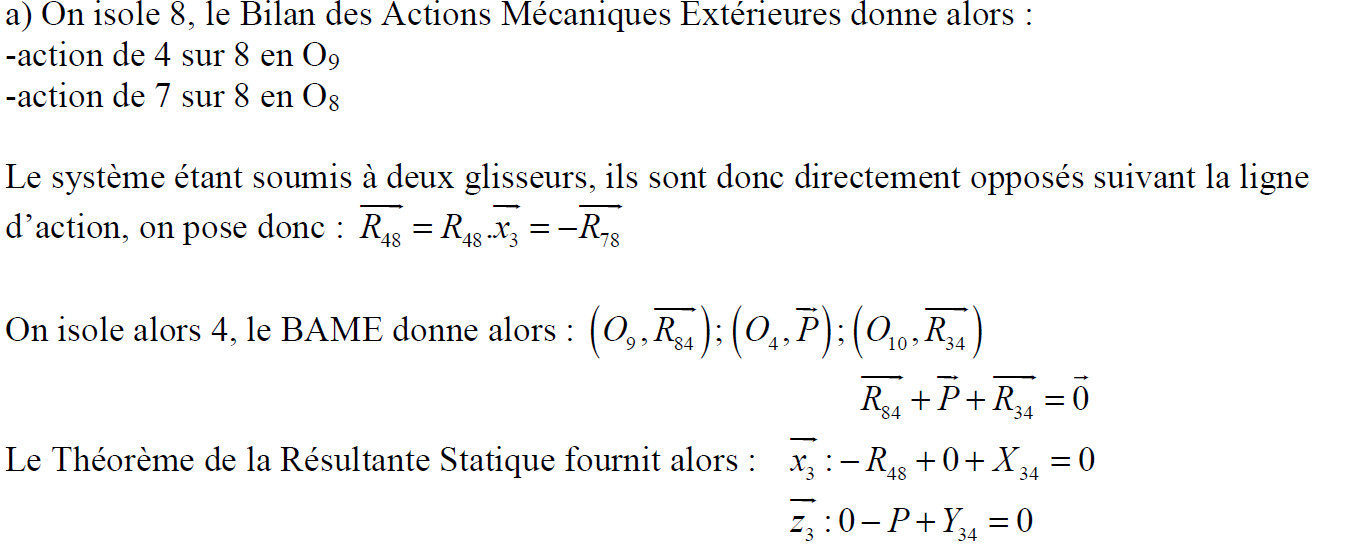
\includegraphics[width=.9\linewidth]{cor_01}
\end{center}

On isole l'ensemble \{(3)+(4)\}. 

On réalise le bilan des actions mécaniques : 
\begin{itemize}
\item action mécanique de (2') sur (3), de direction $\vect{y_2}$;
\item action mécanique de (2) sur (3), de direction $\vect{y_2}$;
\item action mécanique de la pesanteur sur \{(3)+(4)\};
\item action du ressort sur \{(3)+(4)\}.
\end{itemize}

Il faut écrire une équation du PFS permettant de ne pas faire apparaître les actions dans les deux liaisons pivot. Il faut donc réaliser un théorème de la résultante statique en projection sur $\vect{z_2}$ (perpendiculaire à $\vect{y_2}$).

\end{corrige}
\else
\fi

%Q 9. 
\question{\label{q:09}Exprimer l'équation scalaire traduisant l'équilibre du mécanisme en fonction des angles $\alpha$, $\beta$, de la masse $m_{34}$ et de la composante de résultante d'action mécanique $F_{r}$.}
\ifprof
\begin{marginfigure}
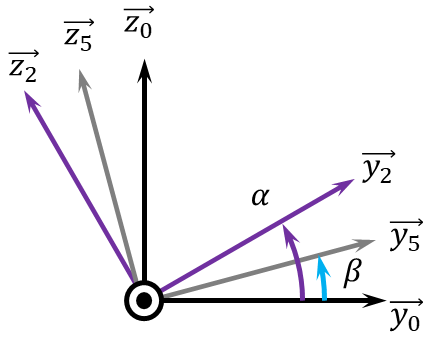
\includegraphics[width=\linewidth]{cor_02}
\end{marginfigure}

\begin{corrige}
Calculons : 
\begin{itemize}
\item la projection de l'action du ressort sur $\vect{z_2}$ : $F_r \vect{y_5} \cdot\vect{z_2}$ $=F_r\cos\left(-\beta +\dfrac{\pi}{2}+\alpha\right)=-F_r\sin\left(\alpha-\beta \right)$;
\item la projection de l'action de pesanteur sur $\vect{z_2}$ : $-m_{34} g \vect{z_0} \cdot\vect{z_2}$ $=-m_{34} g\cos\alpha$.
\end{itemize}
On applique le TRS en projection sur $\vect{z_2}$ et on a  :
$$
\underbrace{\vectf{2'}{3}\cdot \vect{z_2}}_{\vect{0}}+\underbrace{\vectf{2}{3}\cdot \vect{z_2}}_{\vect{0}}+\vectf{\text{Pes}}{3}\cdot \vect{z_2}+\vectf{\text{Res}}{3}\cdot \vect{z_2}=0.
$$

On a donc $-m_{34} g\cos\alpha -F_r\sin\left(\alpha-\beta \right) = 0$ et  
$\boxed{F_r = -m_{34} g \dfrac{\cos\alpha}{\sin\left(\alpha-\beta \right)}}$.



\end{corrige}
\else
\fi

\ifprof
\else
%À partir des relations déterminées précédemment, deux fonctions \texttt{beta(alpha)} et \texttt{effort\_ressort(alpha)} qui renvoient respectivement la valeur de l'angle $\beta$ et la valeur de la composante de résultante d'action mécanique $F_{r}$ sont implantées en Python. La bibliothèque \texttt{numpy} a été importée sous le nom abrégé \texttt{np}. Les variables globales $\mathrm{g}$ et $\mathrm{m} 3$ fournissent respectivement la valeur de l'accélération de la pesanteur terrestre et la valeur de la masse de la nacelle gyrostabilisée (3). Les positions d'équilibre pour différentes valeurs de la masse $m_{4}$ sont alors obtenues par une méthode de recherche de zéro par dichotomie.
\fi

%%Q 10. 
%\question{\label{q:10} Écrire en Python une fonction, \texttt{fonction\_equilibre(m4, alpha)}, qui renvoie zéro lorsque, pour une valeur de masse $m_{4}$ de l'appareil photo donnée, la valeur de l'angle $\alpha$ vaut l'angle d'équilibre recherché.}
%\ifprof
%\begin{corrige} $\quad$
%\begin{lstlisting}
%def fonction_equilibre(m4,alpha):
%    # On donne alpha en radians
%    # beta(alpha) retourne un angle en radians
%    return(effort_ressort(alpha)+(m3+m4)*g*(np.cos(alpha)/np.sin(alpha-beta(alpha))))
%\end{lstlisting}
%
%Cette fonction renvoie 0 si \texttt{alpha} est bien la position d'équilibre.
%
%\end{corrige}
%\else
%\fi

\ifprof
\else
Dès lors, il est posible de tracer l'angle d'équilibre $\alpha_{0}$ en fonction de la masse de l'appareil photo $m_{4}$ (figure~\ref{Cy_11_Ch_03_PFS_2D_TD_05_fig_05}).
%
%Une fonction \texttt{angle\_equilibre(m4)} qui renvoie la valeur de l'angle $\alpha=\alpha_{0}$ correspondant à la position d'équilibre avec une méthode de recherche de zéro par dichotomie est implantée en Python. La courbe obtenue à partir de la fonction \texttt{angle\_equilibre(m4)} représentant l'angle d'équilibre $\alpha_{0}$ en fonction de la masse de l'appareil photo $m_{4}$ est donnée (figure~\ref{fig:05}).
\fi



%\begin{marginfigure}
%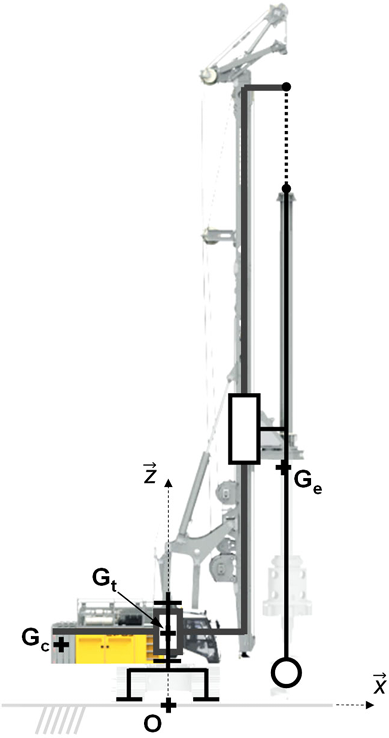
\includegraphics[width=\textwidth]{fig_05}
%\caption{Angle d’équilibre $\alpha_0$ en fonction de la masse de l’appareil photo $m_4$}
%\label{Cy_11_Ch_03_PFS_2D_TD_05_fig_05}
%\end{marginfigure}


\ifprof
\else
\marginnote{
\begin{solution}
\begin{enumerate}
\item $F_r=-F_{r0} - K_r$ $\left(\sqrt{L^2+l^2-2Ll\sin\alpha}-L_{r0}\right)$.
\item ${\vect{F}_{23}=F_{23}\vect{y_2}}$ et ${\vect{F}_{2'3}=F_{2'3}\vect{y_2}}$.
\item .
\item $ZF_r = -m_{34} g \dfrac{\cos\alpha}{\sin\left(\alpha-\beta \right)}$.
\item $-9\degres$ à $18\degres$.  
\end{enumerate}
\end{solution}}
\fi

%Q 11. 
\question{\label{q:11} En donnant les valeurs des angles d'équilibre pour les deux valeurs extrêmes de masse, vérifier le respect de l'exigence 1.1.1. relative à la plage de fonctionnement.}
\ifprof
\begin{marginfigure}
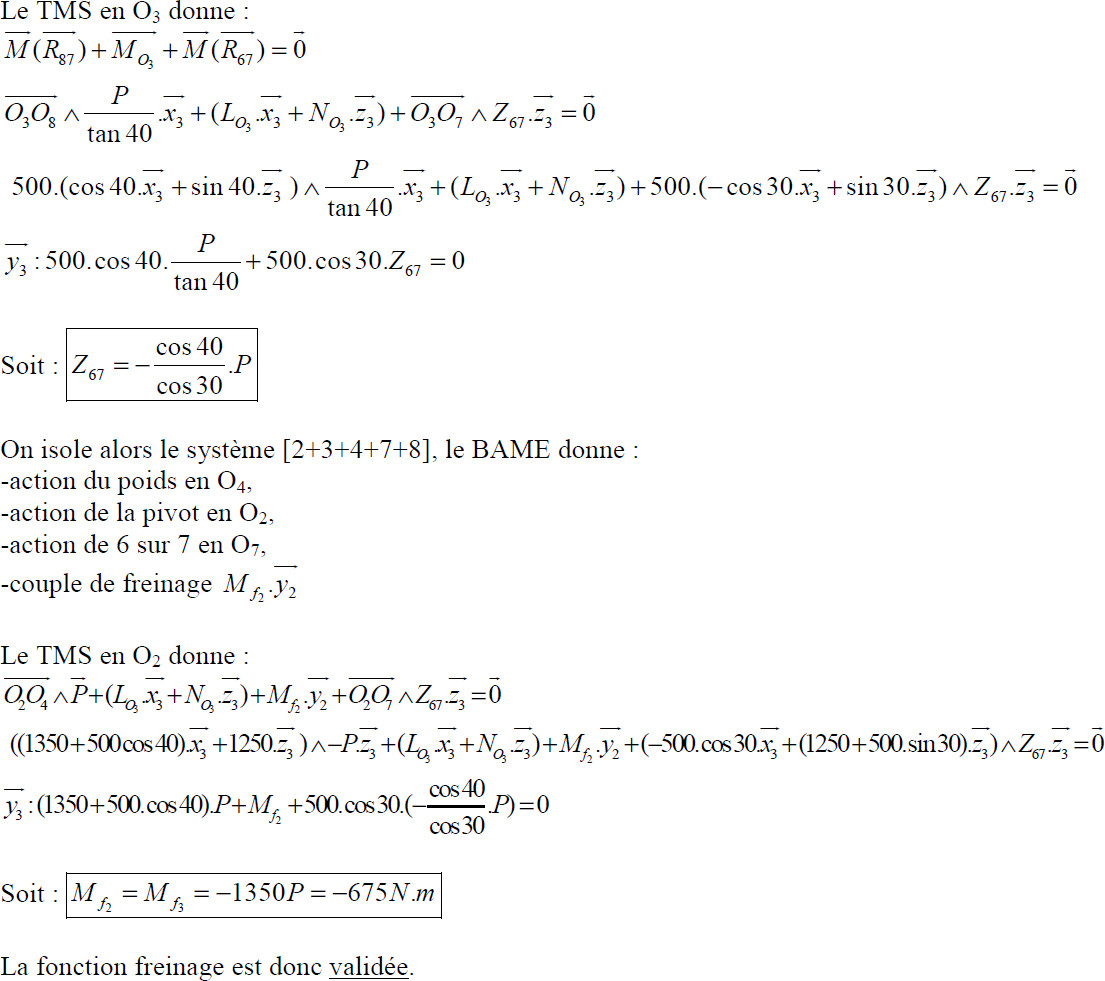
\includegraphics[width=\linewidth]{cor_03}
\end{marginfigure}
\begin{corrige} 

On peut lire en figure \ref{Cy_11_Ch_03_PFS_2D_TD_05_fig_05} que pour une masse d'appareil comprise entre 0,35 et \SI{1,55}{kg}, l'angle d'équilibre varie de $18$ à $-9\degres$. Cet intervalle est compris dans l'intervalle $\left[-35\degres,45\degres\right]$. L'exigence 1.1.1 est donc satisfaite.
\end{corrige}
\else
\fi

\ifprof
\else

\begin{figure}[!h]
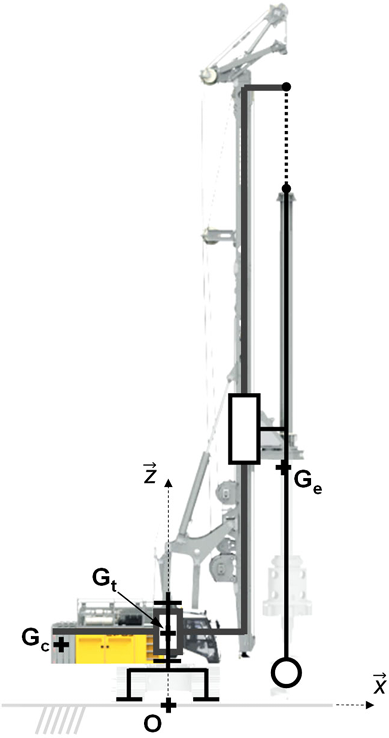
\includegraphics[width=6.5cm]{fig_05}
\caption{Angle d’équilibre $\alpha_0$ en fonction de la masse de l’appareil photo $m_4$}
\label{Cy_11_Ch_03_PFS_2D_TD_05_fig_05}
\end{figure}

\fi

